% arXiv note (DECISIONS #24; plan in writeup/plan.md). Converted from writeup/note.md,
% revision 3; this file is the source from now on. Every number is in results/ with its
% command and commit. Build: bash writeup/make_arxiv.sh. ASCII only: arXiv compiles with
% pdflatex, tectonic (local) with XeTeX.
\documentclass[11pt]{article}
\usepackage[T1]{fontenc}
\usepackage[utf8]{inputenc}
\usepackage{lmodern}
\usepackage[a4paper,margin=1in]{geometry}
\usepackage{amsmath,amssymb}
\usepackage{booktabs}
\usepackage{tabularx}
\usepackage{graphicx}
\usepackage[round]{natbib}
\usepackage{enumitem}
\usepackage[font=small,labelfont=bf]{caption}
\usepackage{microtype}
\usepackage{xcolor}
\definecolor{linkblue}{RGB}{26,82,148}
\usepackage[colorlinks=true,linkcolor=linkblue,citecolor=linkblue,urlcolor=linkblue]{hyperref}

\newcommand{\x}{$\times$}
\newcommand{\rhoeff}{\rho_{\mathrm{eff}}}
\setlist{itemsep=2pt,topsep=4pt}
\emergencystretch=1.5em

\title{Unrolling Integer Activations into Unit Spikes\\
Does Not Save Work:\\
An Exact Accounting on a Ternary Language Model}
% TODO before submission: affiliation and contact e-mail, if any.
\author{Ga\'etan Martin}
\date{}

\begin{document}
\maketitle

\begin{abstract}
Spiking language models report large energy savings, usually by pricing a spike accumulation at
0.9\,pJ against 4.6\,pJ for a 32-bit floating-point multiply-accumulate. Several of them run
integer activations as trains of unit spikes. We measure what that unrolling costs on a model
where it is exact: RWKV-4-169M with ternary weights and 4-bit activations at every projection
input, whose spike engine produces logits bit-identical to its integer engine. On the
projections the usual formula credits spikes with 3.3\x{} less energy; this factors into removed
multiplications (5.1\x) and skipped zeros (1.8\x), both available to an integer engine with
ternary weights, times the cost of the unrolling (0.36). Counted directly, unit spikes need
1.7--3.4 times the accumulations of a zero-skipping integer engine at every site, need fewer
accumulations than a dense engine only at the two sparse sites, and gain nothing from delta
coding; the verdicts hold on TinyStories and WikiText-103. Under every event-driven cost model
we could price, spikes cost more than the integer engine; where weights are held across a
source's spikes, the answer reduces to the cost of a $\pm 1$ increment, which published figures
do not settle.
\end{abstract}

\section{Introduction}

A growing line of work builds language models from spiking neurons and reports large energy
savings: 32.2\x{} for SpikeGPT \citep{zhu2024spikegpt}, 12.9\x{} for SpikeLM
\citep{xing2024spikelm}, 4.76\x{} for SpikingMamba \citep{huang2026spikingmamba}, 6\x{} against an
INT4 model for SDLLM \citep{xu2026sdllm}. Most of these figures come from one formula
\citep{zhou2023spikformer,yao2023sdt}: the spiking network's synaptic operations, firing rate
\x{} time steps \x{} the layer's multiply-accumulates (MACs), are priced at 0.9\,pJ, and the
reference network's MACs at 4.6\,pJ (4.5\,pJ in SpikeGPT). Both are 32-bit floating-point
operations from the 45\,nm table of \citet{horowitz2014}: an addition, and a multiplication plus
addition.

These models differ in what they send per activation (Table~\ref{tab:encodings}). Some send one
binary or ternary spike per step; then each non-zero activation is one event and the spike count
equals the non-zero count. Some send an integer in one graded event, which is an integer engine.
Others unroll an integer into several unit spikes over virtual steps; then a count of 3 becomes
three events.

\begin{table}[t]
\centering\small
\caption{What the cited spiking LMs send per activation.}
\label{tab:encodings}
\begin{tabularx}{\linewidth}{@{}l>{\raggedright\arraybackslash}X>{\raggedright\arraybackslash}X@{}}
\toprule
model & per activation & in the terms of Section~\ref{sec:counting} \\
\midrule
SpikeGPT & binary spikes in the projections, one step per token; $\mathrm{ReLU}^2$ values as
  graded spikes & one event per non-zero value \\
SpikeLM & ternary spikes, one step (headline) or four & one step: one event per non-zero value;
  four: unrolled \\
SpikingMamba & signed multi-level spikes, one step (headline row) & a graded event, or unrolled,
  depending on the hardware \\
SDLLM & integer counts unrolled into bidirectional spikes over 8 steps & unrolled \\
NSLLM \citep{xu2025nsllm} & integer activations expanded into binary spikes over virtual steps
  & unrolled \\
SpikeLLM \citep{xing2025spikellm} & multi-bit neurons, also evaluated expanded into 1-bit spikes
  & both, compared \\
\bottomrule
\end{tabularx}
\end{table}

This note is about the unrolling: given the same integer activations, does sending each as unit
spikes save work over an integer engine? Ternary weights already turn multiplications into
additions \citep{ma2024era}, and accelerators already skip zero activations
\citep{albericio2016cnvlutin,han2016eie,parashar2017scnn}. SpikeLLM already finds, in
bit-operation counts, that expanding its multi-bit neurons into 1-bit spikes costs more
operations. We make the comparison exact and site by site, on a ternary model, against three
integer engines, and look at which cost models could reverse it.

The question has an exact answer when the unrolling is exact, because then the spike engine and
the integer engine compute the same logits and differ only in how many accumulations they
perform and what each costs. We build such a model and:
\begin{itemize}
\item count the accumulations of the unit-spike reading and of three integer engines (dense,
  zero-skipping, delta coding between tokens) on the same weights and inputs, on two corpora
  (Section~\ref{sec:counting});
\item decompose the spiking literature's energy formula on the same model into what spikes
  contribute and what any integer engine already has (Section~\ref{sec:formula});
\item set out which digital cost models make the unrolling pay and which do not
  (Section~\ref{sec:cost}).
\end{itemize}
The verdict bands of Section~\ref{sec:counting} and the cost analysis were fixed in a decision
log kept with the code before the dense, delta and hardware analyses were run; the
zero-skipping ratio $R$ was already known from an earlier measurement on the same checkpoints.

\section{Setting}
\label{sec:setting}

\paragraph{Model.} RWKV-4-169M \citep{peng2023rwkv}: 12 blocks of width 768, each with a time
mix (the WKV recurrence) and a channel mix (a $\mathrm{relu}^2$ MLP of width 3072). Each block
first mixes every token with the previous one, $x_t' = \mu \odot x_t + (1 - \mu) \odot x_{t-1}$
(``token shift''), separately for each projection input ($x_r$, $x_k$, $x_v$). The 84
projections of the blocks become ternary BitLinear layers (92.0\,M parameters): weights in
$\{-1, 0, +1\}$ with one scale per group of 128 inputs, as in BitNet b1.58 \citep{ma2024era}.
Embeddings, the LM head (38.6\,M MACs per token), layer norms, the WKV recurrence and the
sigmoid gates stay in floating point.

\paragraph{Neurons.} Our integer LIF neuron (FAI-LIF), after NSLLM \citep{xu2025nsllm},
quantizes its input to a 4-bit count $q$ per token on a learned grid (LSQ step size
\citep{esser2020lsq}, clipped straight-through gradient) and outputs $s \cdot q$; signed sites
use $q \in [-8, 7]$, the channel-mix $\mathrm{relu}^2$ output $q \in [0, 15]$. The model has 120
of them: one on each of the 7 projection inputs of each block, plus the WKV inputs $k$, $v$ and
the channel-mix output. They are stateless; Appendix~\ref{app:membrane} tests a membrane.

\paragraph{Training and evaluation.} Fine-tuning for 10\,k steps of $16 \times 128$ tokens
(20.5\,M tokens); quantized models add a KL term to the full-precision fine-tuned model.
Perplexity on the first 1\,M tokens of the last 1\% of the corpus, in 128-token windows each
started from a fresh state; two seeds per configuration, on disjoint text
(Table~\ref{tab:configs}).

\begin{table}[t]
\centering\small
\caption{Perplexity of the configurations (mean of 2 seeds). The studied model is the last row.}
\label{tab:configs}
\begin{tabular}{@{}lcc@{}}
\toprule
configuration & TinyStories & WikiText-103 \\
\midrule
full precision, fine-tuned (reference) & 4.986 & 25.44 \\
ternary weights, full-precision activations & 5.157 & -- \\
ternary weights, 4-bit LIF counts at every projection input & \textbf{5.391} (1.081\x)
  & \textbf{35.41} (1.392\x) \\
\bottomrule
\end{tabular}
\end{table}

The converted RWKV-4-169M before fine-tuning reproduces the original (13.98 on TinyStories). The
studied model holds well on TinyStories \citep{eldan2023tinystories} and much less well on
WikiText-103 \citep{merity2016wikitext} at this budget; the counts below do not depend on that
gap.

\section{An exact unrolling}
\label{sec:exact}

A signed count $q \in [-8, 7]$ is unrolled into $|q|$ spikes of sign $\mathrm{sign}(q)$ over
$T = 8$ virtual steps; an unsigned count $q \in [0, 15]$ into $q$ unit spikes over $T = 15$. We
call a site \emph{spike-native} when its consumer is a ternary BitLinear: the 84 projection
inputs. The WKV inputs (whose $e^k$ needs the decoded value) and the channel-mix output
(multiplied by a floating-point gate) are not; they are the same in every engine and are left
out of the counts.

Exactness holds at three levels, which we keep apart:
\begin{enumerate}
\item \textbf{Integer accumulations.} Through a ternary consumer, the accumulations of the
  spikes, summed over steps, equal those of $q$ bit for bit (checked on real counts at every
  spike-native site of blocks 0 and 11, and on random counts in unit tests).
\item \textbf{The whole model, integer against spike engine.} Running all 84 consumers as an
  integer engine (integer accumulation per weight group, then the scales applied once) and as a
  spike engine (the same, with the accumulations taken over the spikes) gives bit-identical
  logits on 4\,k tokens, for both seeds.
\item \textbf{Against the floating-point training graph.} Both engines match it only up to float
  rounding, which a downstream LIF can turn into a different count: cross-entropy within 0.05\%,
  98--99\% of argmaxes equal.
\end{enumerate}
The accounting compares levels 1--2: two engines computing the same function. The counts of
Section~\ref{sec:counting} are taken on the floating-point graph's trace; recounted on the integer
engine's own trace, where a downstream count can differ (level 3), every ratio quoted in this note
changes by at most 0.0012 (0.01\% relative), and no displayed value or verdict changes.

The change between consecutive tokens, $\Delta q_t = q_t - q_{t-1}$, lies in $[-15, 15]$ and is
unrolled the same way on a signed 5-bit grid ($T = 16$). A consumer that keeps its previous
output computes $y_t = y_{t-1} + W \Delta q_t = W q_t$ exactly.

\section{Counting accumulations}
\label{sec:counting}

For a ternary consumer $W$ (out \x{} in) and the counts $q_i$ of one token, let
$c_i = \mathrm{nnz}(W_{:,i})$. Weight zeros are static and every engine below skips them (an
engine that does not multiplies all counts by 1.47). The accumulations per token are in
Table~\ref{tab:engines}.

\begin{table}[t]
\centering\small
\caption{Accumulations per token of a ternary consumer, by engine.}
\label{tab:engines}
\begin{tabular}{@{}lll@{}}
\toprule
engine & accumulations & operand \\
\midrule
D, dense activations & $\sum_i c_i$ & 4-bit count \\
Z, zero activations skipped & $\sum_i \mathbf{1}[q_i \neq 0]\, c_i$ & 4-bit count \\
S, unit spikes & $\sum_i \lvert q_i \rvert\, c_i$ & one spike \\
$\Delta$Z, $\Delta$S & Z, S on $\Delta q_t$ & 5-bit count, one spike \\
\bottomrule
\end{tabular}
\end{table}

\paragraph{Cost per accumulation.} Every engine accumulates per weight group, as the integer
path of a BitLinear does: with 128 inputs per group, ternary weights and counts of magnitude at
most 15 (including $\Delta q$), a group sum is at most $128 \times 15 = 1920$ in magnitude and
fits a 12-bit signed accumulator (the largest we observe is 348). The group's scale is then
applied once in floating point, the same in every engine, and is left out of the counts. Let $a$
be the cost of adding a 4-bit operand into that accumulator and $\rho a$ that of a $\pm 1$
increment of it. Counting additions only, the unit spikes are cheaper than engine X when
$\rho < \rho^* = \mathrm{ops}_X/\mathrm{ops}_S$. Section~\ref{sec:cost} adds the cost $f$ of
reading the weight. We examine two reference pricing assumptions for $\rho$, not physical bounds.
Both operands enter the same 12-bit adder, and Horowitz's table prices additions by width:
$\rho = 1$. Priced by operand width instead, an assumption favourable to spikes: $\rho = 1/4$.
The bands: $\rho^* > 1$, unit spikes need fewer accumulations and are cheaper under both
pricings; $\rho^* < 1/4$, dearer under both; in between, the verdict depends on the pricing.

\paragraph{The sign is trivial, the size is not.} $|q_i| \geq \mathbf{1}[q_i \neq 0]$, so
$R = S/Z \geq 1$ for any network, with equality when every non-zero count is $\pm 1$, as with
one-step binary or ternary spikes. What a measurement adds is how far above 1 unrolling puts it:
the mean count of a non-zero activation is 1.7 at the sparse time-mix output, 2.2 at the
$\mathrm{relu}^2$ output, 2.6 to 3.1 at the dense projection inputs.

\paragraph{Results.} Table~\ref{tab:results} gives the counts on TinyStories (first 256 windows
of the evaluation tail, 32\,k tokens) and Figure~\ref{fig:rho} the same numbers on a log scale.

\begin{table}[t]
\centering\footnotesize
\setlength{\tabcolsep}{4pt}
\caption{Break-even ratios on TinyStories, per spike-native site pooled over the 12 blocks; a
range gives the two seeds. They agree to within 0.06 in $\rho^*$, except 14.3 against 15.3 at
the $\mathrm{relu}^2$ site against D.}
\label{tab:results}
\begin{tabular}{@{}lcccccc@{}}
\toprule
site & non-zero & $E\lvert q\rvert$ & $\rho^*$ vs D & $\rho^*$ vs Z ($=1/R$)
  & $\rho^*$ $\Delta$S vs $\Delta$Z & $\Delta$Z\,/\,Z \\
\midrule
channel-mix $\mathrm{relu}^2$ output $\to W_v$ & 3\% & 0.07 & 14.3--15.3 & 0.45--0.46
  & 0.50--0.51 & 1.56--1.58 \\
time-mix output $\to W_o$ & 17--18\% & 0.30 & 3.3 & 0.57--0.58 & 0.62 & 1.25 \\
time-mix input $x_r \to W_r$ & 83\% & 2.16--2.17 & 0.46 & 0.38 & 0.37 & 1.01 \\
time-mix input $x_k \to W_k$ & 84\% & 2.23--2.24 & 0.44--0.45 & 0.38 & 0.35 & 1.00 \\
time-mix input $x_v \to W_v$ & 87\% & 2.71--2.72 & 0.37 & 0.32 & 0.27 & 1.01 \\
channel-mix input $x_k \to W_k$ & 86\% & 2.52--2.55 & 0.39--0.40 & 0.34 & 0.34--0.35 & 0.98 \\
channel-mix input $x_r \to W_r$ & 82--84\% & 2.13--2.19 & 0.46--0.47 & 0.38--0.39 & 0.38
  & 0.99 \\
\midrule
\textbf{pooled} & & & \textbf{0.65} & \textbf{0.36} & \textbf{0.35} & \textbf{1.01} \\
\bottomrule
\end{tabular}
\end{table}

\begin{figure}[t]
\centering
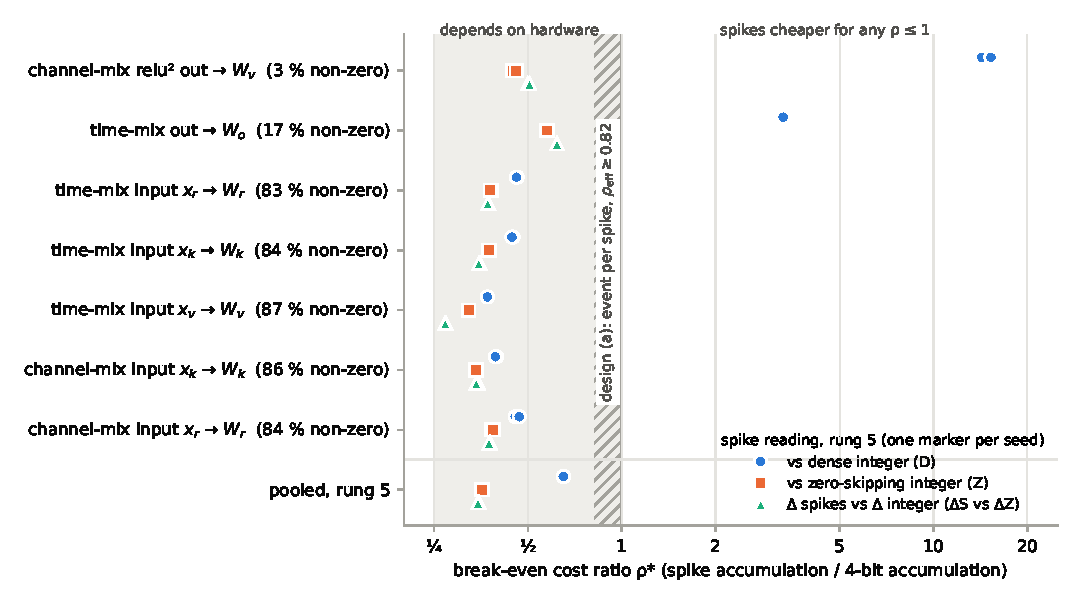
\includegraphics[width=\linewidth]{figures/rho_star.pdf}
\caption{Break-even cost ratio $\rho^*$ per spike-native site of the studied model on
TinyStories, pooled over the 12 blocks (one marker per seed). Unit spikes are cheaper than an
integer engine when a spike accumulation costs less than $\rho^*$ times a 4-bit accumulation.
Shaded: between the two reference pricings, $\rho = 1/4$ and $\rho = 1$. Hatched: design (a)
of Section~\ref{sec:cost}, $\rhoeff \geq 0.82$.}
\label{fig:rho}
\end{figure}

\begin{itemize}
\item \textbf{Against Z, unit spikes always need more accumulations:} $R$ = 1.7 to 3.1 per site
  (up to 3.4 at twice the training budget), 2.8 pooled. A $\pm 1$ increment would have to cost
  between 0.32 and 0.58 of a 4-bit addition.
\item \textbf{Against D, the verdict follows sparsity.} At the two sparse sites unit spikes
  need fewer accumulations ($\rho^*$ = 3.3 and 14--15), so they are cheaper under both
  pricings. At the five dense input sites, which carry 61.5\% of the projection work, and pooled
  ($\rho^* = 0.65$), they need more, and are cheaper only if a $\pm 1$ increment costs less than
  $\rho^*$ (0.37--0.47 per site) of a 4-bit addition, as under operand-width pricing. Z gets the
  sparse sites' benefit without the unrolling.
\item \textbf{Delta coding saves nothing.} At the dense sites $\Delta q$ is non-zero as often as
  $q$; at the sparse sites more often, since a unit that turns on and off makes two changes. The
  bands are the same as without it, except one site of the model trained at twice the budget,
  which becomes ``dearer''.
\end{itemize}

\paragraph{Neuron sites only.} On TinyStories, the model with 4-bit counts only at the neuron
sites (the WKV inputs, the two sparse sites and the channel-mix output), whose only spike-native
sites are the two sparse ones, gives a pooled $\rho^*$ of 8.8--8.9 against D and 0.53 against Z.

\paragraph{WikiText-103.} Retrained and counted the same way, no site changes band in any of
the three comparisons: pooled $\rho^*$ 0.68--0.69 against D, 0.37--0.38 against Z
($R$ = 2.66--2.69), 0.36 for $\Delta$S against $\Delta$Z.

\paragraph{Sparser training.} The quantizers were not trained for sparsity. A firing-rate
penalty would lower the counts: it can turn a 3 into a 1, which lowers S and leaves Z unchanged,
so it can lower $R$ and raise $\rho^*$ against Z, towards 1 but never above it ($S \geq Z$ holds
for any counts). It would also change perplexity; neither effect is measured here.

\section{What the spiking energy formula counts}
\label{sec:formula}

Applied to the studied model as Spikformer and Spike-driven Transformer apply it (synaptic
operations $= E|q| \times$ MACs at 0.9\,pJ, against the same MACs at 4.6\,pJ for the
full-precision network), the formula gives the spiking model 3.3\x{} less energy on the
projections (3.5\x{} on WikiText-103), 2.0\x{} with the full-precision LM head counted on both
sides. On the spike-native layers the ratio factors exactly, with $M_s$ the MACs and $P_s$ the
non-zero fraction of site $s$:
\begin{equation}
\frac{E_{\mathrm{ANN}}}{E_{\mathrm{SNN}}}
= \frac{4.6}{0.9} \times \frac{\sum_s M_s}{\sum_s P_s M_s}
\times \frac{\sum_s P_s M_s}{\sum_s E|q|_s M_s},
\end{equation}
which on TinyStories is 5.11 (multiplications removed) \x{} 1.82 (zeros skipped) \x{} 0.36
(unrolling). The first two factors are what ternary weights and zero skipping give any engine:
an integer engine that skips zeros, priced with the same constants, gets
$5.11 \times 1.82 = 9.3\times$ ($13.7\times$ if it also skips weight zeros, which the formula
does not count). The third is the unrolling's own contribution, and it is a cost. For one-step
binary or ternary spikes the third factor is 1, and the whole saving is the first two.

The constants are FP32 operations. The 12-bit integer additions of Section~\ref{sec:counting}
lie between the 8- and 32-bit rows of the same table (0.03 and 0.1\,pJ), a further 9--30\x{}
that integer and spike engines could both claim. When the reference network is itself integer,
charging its operations the FP32 MAC constant hands the spiking side the 5.1\x{} of the
constants: SDLLM reports 6\x{} less energy than an INT4 model while performing 1.15\x{} fewer
operations (our arithmetic from its Table~2).

\section{Cost models}
\label{sec:cost}

Whether the unrolling pays depends on what an accumulation costs besides the addition, above all
on how often the weight is read. We consider two designs.

\paragraph{(a) One event per spike, weight read per event.} This is how event-driven chips
process spikes: each accumulation reads the weight it adds, at cost $f$. From the smallest SRAM in
Horowitz's table (10\,pJ per 64-bit read), 32 packed ternary weights cost $f \approx 0.31$\,pJ
each, 3 to 10 times a 12-bit addition, which lies between the 8- and 32-bit rows ($a$ =
0.03--0.1\,pJ; the upper end, the most favourable to spikes, overstates it). Unit spikes are
cheaper than Z only if $\rhoeff = (\rho a + f)/(a + f) < 1/R$; here $\rhoeff$ is 0.82 to 0.93
even at $\rho = 1/4$, about 0.91 if $a$ grows linearly with width from the 8-bit row.
The per-event model of \citet{davidson2021}, from SpiNNaker~2 post-layout figures, reaches the
same: with $E$ the cost of an addition, a weight read costs about $5E$, a spike event $7E$, a
multiply-accumulate event $12E$; without the multiplication, which ternary weights remove, an
integer event also costs $7E$. Published per-event energies (23.6\,pJ minimum, simulated, on
Loihi \citep{davies2018loihi}; 26\,pJ with static power on TrueNorth
\citep{merolla2014truenorth}; 10--20\,pJ on SpiNNaker~2 \citep{hoppner2021spinnaker2}) are 100
to 900 times a 45\,nm addition. They come from different chips and do not give the ratio between
the two engines on any one of them, but they show that an event's cost is dominated by memory,
routing and the neuron update rather than by the width of what it carries. Loihi~2 sends integer
payloads in one ``graded'' spike at what Intel calls negligible extra energy over a binary spike
\citep{intel2021loihi2}, a qualitative indication that one event per count costs about the same
as one event per unit.

\paragraph{(b) Weight held across a source's spikes.} If the engine reads the weight once and
applies all $|q_i|$ unit spikes of input $i$ from a register, the read is paid once per non-zero
input in both engines ($Zf + S\rho a$ against $Z(f + a)$) and drops out. Unit spikes are then
cheaper than Z if and only if $\rho < 1/R$: a $\pm 1$ increment of the 12-bit group accumulator
must cost less than 0.29 to 0.58 of adding a 4-bit operand into it. Horowitz prices additions by
width ($\rho = 1$, no); pricing by operand width ($\rho = 1/4$, yes) is an assumption. We found
no published figure that settles it.

\begin{table}[t]
\centering\footnotesize
\caption{Verdict of unit spikes under each cost model: cheaper or dearer than the integer engine.
The two reference pricings count additions only.}
\label{tab:cost}
\begin{tabular}{@{}llccc@{}}
\toprule
cost model & $\rho$ or $\rhoeff$ & vs Z & vs D, sparse sites & vs D, input sites \\
\midrule
operand-width pricing & 1/4 & cheaper & cheaper & cheaper \\
adder-width pricing (Horowitz, 45\,nm) & 1 & dearer & cheaper & dearer \\
(a) event per spike, weight read from SRAM & 0.82--1 & dearer & cheaper & dearer \\
(a) per-event model, SpiNNaker~2 figures & $\approx 1$ & dearer & cheaper & dearer \\
(b) weight held across a source's spikes & adder $\rho$ & open & cheaper & open \\
\bottomrule
\end{tabular}
\end{table}

Under every design (a) model we could price, unit spikes cost more than a zero-skipping integer
engine at every site (Table~\ref{tab:cost}). Under design (b) the verdict is the cost of a
$\pm 1$ increment, which these figures leave open. These are cost models, not a bound on digital
hardware.

\paragraph{The whole model.} The projections are a small part of a token's energy. With the LM
head in FP16 (58\,\textmu J per token at 1.5\,pJ per MAC), their additions cost
1.0--3.4\,\textmu J in Z and 2.9--9.6\,\textmu J in S at $\rho = 1$ ($a$ = 0.03--0.1\,pJ), so
the reading moves a token's arithmetic by $-2\%$ to $+10\%$; under design (a) weight reads add
10.7\,\textmu J (Z) or 30\,\textmu J (S). If the 23\,MB of ternary weights come from DRAM at
batch 1, moving them costs 7 to 125 times the arithmetic. These are orders of magnitude, not the
cost model of a built engine. The spiking LMs cited above also keep a floating-point head.

\section{Related work}
\label{sec:related}

\paragraph{Spiking language models.} SpikeGPT, SpikeLM, SpikeBERT \citep{lv2023spikebert},
SpikingMamba and SDLLM estimate energy with the 0.9\,/\,4.6\,pJ constants (4.5\,pJ in SpikeGPT)
against a different, full-precision or INT4 reference network; SpikingBERT
\citep{bal2024spikingbert} uses the same constants against the same architecture run without
spikes. SpikeLLM counts bit operations instead and finds that expanding its multi-bit neurons
into 1-bit spikes costs more operations than the multi-bit execution; our accounting is that
comparison made exact and site by site, with ternary weights and integer baselines. NSLLM, whose
integer-to-binary inference our neuron follows, reports a 19.8\x{} ratio of dynamic power between
an FPGA and a GPU.

\paragraph{Fair accounting of spiking networks.} \citet{davidson2021} show that on digital
hardware a rate-coded spiking network wins only below about 1.7 spikes per output, because
weight and state memory accesses dominate. \citet{dampfhoffer2022} include memory accesses and
compare with 16- and 8-bit accelerators, including zero-skipping ones, and attribute any spiking
advantage to spike sparsity rather than to replacing MACs with accumulations;
\citet{lemaire2022} also find memory dominant. None compares one network under both executions,
or against a ternary integer engine that skips zeros.

\paragraph{Integer engines.} Ternary weights remove the multiplications \citep{ma2024era}.
BitNet a4.8 \citep{wang2024bitneta48} runs 4-bit activations on them for the attention and FFN
input projections, keeping the others at 8 bits with sparsification; our model takes every
projection input to 4 bits. Cnvlutin \citep{albericio2016cnvlutin}, EIE \citep{han2016eie} and
SCNN \citep{parashar2017scnn} skip zero activations or weights in hardware. Delta networks
\citep{neil2017delta} and sigma-delta networks \citep{oconnor2016sigmadelta} propagate only
changes; here the changes are as dense as the values.

\section{Limits}
\label{sec:limits}

\begin{itemize}
\item One model (RWKV-4-169M) at one size, two corpora; counts on 32\,k tokens per checkpoint.
  The conversion's quality depends on the corpus (1.08\x{} on TinyStories, 1.39\x{} on
  WikiText-103 at the same budget); the accounting does not.
\item The result concerns unrolling integer counts into unit spikes through stateless consumers.
  One-step binary or ternary spikes have $R = 1$ and keep only the first two factors of
  Section~\ref{sec:formula}; graded spikes are the integer engine. A network whose neurons
  integrate spikes over time steps computes a function of spike timing and has no integer twin
  of this kind.
\item Digital cost models only; analog or in-memory substrates price accumulation differently.
  Design (b) rests on the cost of a $\pm 1$ increment, not measured here.
\item Quantizers not trained for sparsity (Section~\ref{sec:counting}).
\end{itemize}

\section{Conclusion}

When a quantized language model's integer activations are unrolled into unit spikes, the same
network runs as an integer engine, and the comparison is about work rather than about models.
Here the unrolling never needs fewer accumulations than an integer engine that skips zeros,
needs fewer than a dense engine only where activations are sparse, and gains nothing from delta
coding, on two corpora. Under event-driven cost models that read a weight per spike it costs
more; where weights are held across a source's spikes it can pay only if a $\pm 1$ increment
costs well under a 4-bit addition, which we could not establish. The savings reported for such
models come from removing multiplications and skipping zeros, which an integer engine with
ternary weights also has, priced with FP32 constants. Unless a $\pm 1$ increment costs well
under a 4-bit addition, unit spikes can pay in such a model only at the sparse sites, and even
there an integer engine that skips zeros needs $R$ times fewer accumulations.

\appendix

\section{The membrane}
\label{app:membrane}

A LIF neuron differs from a quantizer by its membrane, the residual of one token carried with
leak $\beta$ into the next. On the model with 4-bit counts at the neuron sites only (PPL 5.328 on
TinyStories), we trained the same configuration with a membrane, its gradient through time
detached because it explodes (\x30 per block backward), so $\beta$ learns from its effect within
one token only. Started at $\beta = 0.9$ with a small learning rate, $\beta$ barely moved
(0.87--0.90) and the perplexity was 5.543 ($+4.0\%$); trained at the model's learning rate,
$\beta$ spread over 0.03--0.95 and the perplexity was 5.523 ($+3.7\%$); the pre-registered
threshold to keep the membrane was 5.062. Setting $\beta = 0$ at evaluation changes either
model's perplexity by $-0.02\%$ to $-0.4\%$. No benefit was observed under our detached-state
training protocol; this does not test a membrane trained through time.

\section{Reproduction}
\label{app:repro}

Code, decision log (DECISIONS \#15--\#24) and results:
\url{https://github.com/Orolol/SpikeBit}. Repository names
of the configurations: rung 1 (full precision), rung 2 (ternary weights), rung 3 (4-bit counts
at the neuron sites), rung 5 (studied model), rungs 4b and 4c (membrane).
\begin{itemize}
\item Training and perplexities: \nolinkurl{results/stage_a_ladder.md} (commands, commits,
  checkpoints); WikiText-103 runs: \nolinkurl{colab/ladder_general.py}.
\item Counts: \nolinkurl{scripts/spike_accounting.py} on the checkpoints, with
  \texttt{CORPUS=wikitext103} in the environment for WikiText-103, and \texttt{ENGINE=integer}
  for the integer engine's trace (compared by \nolinkurl{scripts/accounting_engines.py}); tables by
  \nolinkurl{scripts/accounting_tables.py}; Figure~\ref{fig:rho} by
  \nolinkurl{scripts/accounting_figure.py}.
\item Exactness: unit tests in \nolinkurl{src/spiking_ternary_lm/neurons/tests/test_binary_lif.py}
  (spike and delta readings through a ternary BitLinear); whole-model check
  \nolinkurl{scripts/spike_logits_check.py}.
\item Cost models and their sources: \nolinkurl{results/hardware_cost_note.md}.
\item Membrane: \nolinkurl{scripts/_beta_stats.py}, \nolinkurl{scripts/_diagnose_state_regime.py}.
\end{itemize}

\bibliographystyle{plainnat}
\bibliography{refs}

\end{document}
